\documentclass[
        11pt,
        compress,
        xcolor={dvipsnames}
    ]{beamer}

\usetheme[progressbar,sectionpages]{bergen}
%%%%%%%%%%%%%%%%%%
% Font settings
%%%%%%%%%%%%%%%%%%
%\usepackage{tgpagella}
\usepackage[osf]{newpxtext}
\linespread{1.05}
\usepackage[T1,euler-digits]{eulervm}
\usepackage[scaled=0.85]{beramono}
\usepackage[T1]{fontenc}      % Activate Type 1 fonts
\usepackage[utf8]{inputenc} % We want æøå
\usepackage{textcomp}
\usepackage{anyfontsize}
\usepackage[protrusion=true,expansion=true]{microtype}
\usepackage{textcase}
\usefonttheme{serif}
\usefonttheme{professionalfonts}
\usepackage{fourier}
%%%%%%%%%%%%%%%%%%
% General packages
%%%%%%%%%%%%%%%%%%
\usepackage[english]{babel}    % language
\usepackage{xspace}
\usepackage{verbatim}   % at least use begin{comment} end{comment}
\usepackage{booktabs}   % Publication quality tables
\usepackage{graphicx}
\usepackage{bmpsize}    % Handles figures
\usepackage{subcaption}
\usepackage{wrapfig}
% Change the default alignment of a image from left or right an easy manner:
\usepackage[export]{adjustbox}
\usepackage[final]{pdfpages}
\usepackage{multirow,multicol}
\usepackage{array}
% caption for figures
\usepackage{caption}
\captionsetup[figure]{labelfont={bf},labelformat={default},labelsep=colon,name={Fig.}}
\captionsetup[table]{labelfont={bf},labelformat={default},labelsep=colon,name={Table}}
\captionsetup{compatibility=false}
\usepackage{alltt}
\usepackage{forloop}               % For-loops!
\usepackage[numbers,sort&compress]{natbib} % Sort numerical keys for multiple cites
\usepackage{hypernat}       % Avoid breaking 'backref' option of hyperref package
\usepackage{float}
\usepackage{units}                % semantically represent numbers with units
\usepackage{url}
\usepackage{emptypage} % remove head and foot for empty pages
\usepackage[object=vectorian]{pgfornament}
\usepackage{fontawesome5}
\usepackage{import}
\usepackage{fnpct}
\usepackage[absolute,overlay]{textpos}

% Tikz/PGF
%%%%%%%
\usepackage{tikz}
\usetikzlibrary{positioning,shapes.geometric}
\usetikzlibrary{arrows,automata}
\usetikzlibrary{fit}
\usetikzlibrary{topaths}
\usetikzlibrary{patterns}
\usetikzlibrary{calc,decorations}
\usetikzlibrary{decorations.text,decorations.pathmorphing,decorations.pathreplacing}
\usetikzlibrary{matrix}
\usetikzlibrary{shapes}

\usepackage{pgf}
\usepackage{pgfplots}
\pgfplotsset{compat=1.18}
\pgfdeclarelayer{background}
\pgfdeclarelayer{foreground}
\pgfsetlayers{background, main, foreground}

\tikzstyle{every picture}+=[remember picture]

%%%%%%%%%%%%
% Theorems & Math & Algorithms
%%%%%%%%%%%%
\usepackage{amsthm}
\usepackage{thmtools}

\usepackage{amsmath}
\usepackage{mathtools}
\usepackage{amssymb}
\usepackage{amsfonts}
\usepackage{latexsym}

\usepackage{algorithm}
\usepackage[noend]{algpseudocode}

%%%%%%%%%%%%
% Listings
%%%%%%%%%%%%
\usepackage[procnames]{listings} % beautiful listings
\lstdefinelanguage{ansible}
{
    basicstyle=\ttfamily\footnotesize,
    captionpos=b,
    showtabs=false,
    tabsize=4,
    columns=fullflexible,
    % framexleftmargin=10pt,
    % xleftmargin=.03\textwidth,
    % numberstyle=\scriptsize,
    numbersep=4pt,
    % frame=single,
    xleftmargin=\parindent,
    breaklines=true,
    keepspaces=true,
    showspaces=false,
    showstringspaces=false,
    breakatwhitespace=false,
    backgroundcolor=\color{white},
    identifierstyle=\color{black},
    morestring=[s]{"}{"},
    stringstyle=\color{OliveGreen},
    comment=[l]{//},
    morecomment=[s]{/*}{*/},
    commentstyle=\color{OliveGreen},
    keywordstyle={[1]\bfseries\color{Maroon}},
    keywordstyle={[2]\color{RoyalBlue}},
    keywordstyle={[3]\color{BlueGreen}},
    keywords=[1]{include_tasks,import_role,name,when,become}
}

% For comments:
% Use notes/todonotes for comments
\usepackage{xargs}  % Use more than one optional parameter in a new commands
\usepackage[colorinlistoftodos,prependcaption,textsize=small,textwidth=2cm]{todonotes}
\setlength{\marginparwidth}{2cm}
\newcommandx{\notes}[2][1=]{\todo[linecolor=blue,backgroundcolor=blue!25,bordercolor=blue,#1]{#2}}

% Use com for comments
\usepackage{comment}
\newcommand{\com}[1]{
        \mbox{}
       \marginpar{\hrule\footnotesize\raggedright\hspace{0pt}#1\vspace{2mm}}
}
\newcommand{\rui}[1]{\textcolor{OliveGreen}{#1}}

\definecolor{links}{HTML}{2A1B81}
\hypersetup{colorlinks,linkcolor=,urlcolor=links}


\title[LLM-Based NER System]{\large LLM-Based NER System for Medieval Historical Texts\\[0.2em]\small Architecture, Runtime Modes, and Engineering Results}
\author[\underline{Wang}]%
{\texorpdfstring{\underline{\textbf{Rui Wang}}\inst{1} \newline \small \url{rwa041@uib.no} \\[0.1cm] }
  {R. Wang}}

\institute{
  \textbf{\inst{1} Digital development group, education and research support section,
    \newline \hspace{0.2cm}
    \vspace{0.3cm}
  University of Bergen Library, Bergen, Norway \newline
  }
}

\date[AI-NER]{15.04.2026}

\setbeamertemplate{footline}[frame number]{}
\setbeamercovered{transparent=16}

\newcommand{\slidefig}[2][0.7\textheight]{%
  \begin{center}
    \includegraphics[width=\textwidth,height=#1,keepaspectratio]{#2}
  \end{center}
}

\newcommand{\halfslidefig}[2][0.56\textheight]{%
  \begin{center}
    \includegraphics[width=\linewidth,height=#1,keepaspectratio]{#2}
  \end{center}
}

\begin{document}

\begin{frame}[plain]
	\titlepage
\end{frame}


\begin{frame}{Agenda}
  \tableofcontents[hideallsubsections]
\end{frame}

\section{Problem and Motivation}

\begin{frame}{What Is Named Entity Recognition?}
  \begin{itemize}
    \item Named Entity Recognition (NER) is a Natural Language Processing (NLP) task to
    identify and classify named entities in unstructured text data.
    \item It classifies these entities into categories such as person, place, organization, etc.
    \item For historical research, NER is a first step for information extraction across large text corpora — identifying who was mentioned, where, when, and in what role.
  \end{itemize}
\end{frame}

\begin{frame}{NER in This Project}
  \begin{columns}[T]
    \begin{column}{0.55\textwidth}
      \begin{itemize}
        \item In this project, one CSV row is one historical record to process.
        \item The system reads the raw record text from the \texttt{Tekst} field.
        \item It then produces annotated text plus structured entity metadata.
        \item More than 18000 records need processing, so automation is essential.
      \end{itemize}
    \end{column}
    \begin{column}{0.45\textwidth}
      \begin{block}{Sample Input CSV}
        \scriptsize
        \textbf{Header:}\\
        "Bindnr";"Brevid";"Tekst"\\[0.4em]
        \textbf{Example row:}\\
        "1";"601";"Ollum monnum þæim sæm þetta bref sea æder højra sændir Olauer med gudz nadh abote \ldots"
      \end{block}
      \vspace{0.2cm}
      \scriptsize
      The NER step must recognize entities inside this long historical text and
      return them in a reusable structured format.
    \end{column}
  \end{columns}
\end{frame}

\begin{frame}{Why This Project Is Difficult}
  \begin{itemize}
    \item The source material is medieval historical text: spelling varies, text styles differ, and languages mix.
    \item Large historical corpora: manual annotation is infeasible, and error-prone for non-experts.
    \item Domain expertise is needed to understand context and annotate entities correctly.
    \item Existing NER tools might struggle with unstandardized and mixed-language input.
    \item LLMs are an option to handle complex language patterns at scale, but their outputs still require careful prompting, validation, and post-processing.
  \end{itemize}
\end{frame}

\begin{frame}{Operational Challenges}
  \begin{itemize}
    \item Corpus file with more than 18000 historical text records.
    \item At scale, baseline per-record API processing and sequential execution become time-consuming.
    \item API-backed processing also has direct monetary cost, so prompt shape and execution mode matter.
    \item Concurrency and batch execution improve scalability, but they also add orchestration complexity.
    \item The system must balance throughput, cost, concurrency limits, failure handling, and output ordering.
  \end{itemize}
\end{frame}

\begin{frame}{Python Async Concurrency}
  \scriptsize
  \begin{block}{Core Idea: Concurrency}
    It means a program can make progress on multiple tasks during the same
    period by switching when one task is waiting. This helps I/O-bound work such as
    network requests, but it is not the same as multi-core parallelism.
  \end{block}
  \vspace{0.3em}
  \begin{block}{Key Terms in Python}
    \begin{itemize}\setlength{\itemsep}{0.3em}
      \item \textbf{Coroutine}: an \texttt{async def} function that can pause at \texttt{await}.
      \item \textbf{Task}: a scheduled coroutine managed by the event loop.
      \item \textbf{Event loop}: the \texttt{asyncio} runtime that switches between waiting tasks.
    \end{itemize}
  \end{block}
  \vspace{0.3em}
  \scriptsize
  This project uses \texttt{asyncio} from the Python standard library to overlap
  LLM calls, batch polling, and fallback processing.
\end{frame}

\begin{frame}[shrink=2]{Batch Processing and Claude Message Batches API}
  \begin{columns}[T]
    \begin{column}{0.48\textwidth}
    \scriptsize
      \begin{block}{Core Idea: Batch Processing}
        It submits many requests together for asynchronous processing.
        It is useful when immediate responses are not required and throughput or cost matters more than per-request latency.
      \end{block}
      \vspace{0.3em}
      \begin{block}{Message Batches API}
        \begin{itemize}\setlength{\itemsep}{0.3em}
          \item The system creates a Message Batch with a list of requests.
          \item Each request is processed asynchronously and handled independently by Claude.
          \item The status of the batch can be polled and results can be retrieved when processing has ended for all requests.
          \item Results are not guaranteed to come back in input order, so \texttt{custom\_id} is used to match them back.
        \end{itemize}
      \end{block}
    \end{column}
    \begin{column}{0.52\textwidth}
      \begin{block}{Python SDK Structure}
        \ttfamily\tiny
        batch = client.messages.batches.create(\\
        \hspace*{1em}requests=[\\
        \hspace*{2em}\{\\
        \hspace*{3em}"custom\_id": "record-601",\\
        \hspace*{3em}"params": \{ model, max\_tokens,\\
        \hspace*{5em}messages: [\{...\}] \}\\
        \hspace*{2em}\},\\
        \hspace*{2em}\{\\
        \hspace*{3em}"custom\_id": "record-602",\\
        \hspace*{3em}"params": \{ ... \}\\
        \hspace*{2em}\}\\
        \hspace*{1em}]\\
        )
      \end{block}
      \vspace{0.3em}
      \begin{block}{Runtime Pattern}
        \scriptsize
        \texttt{create batch $\rightarrow$ poll status $\rightarrow$ fetch results}
      \end{block}
    \end{column}
  \end{columns}
\end{frame}

\section{How the System Is Structured}

\begin{frame}{System Architecture Overview}
  \centering
  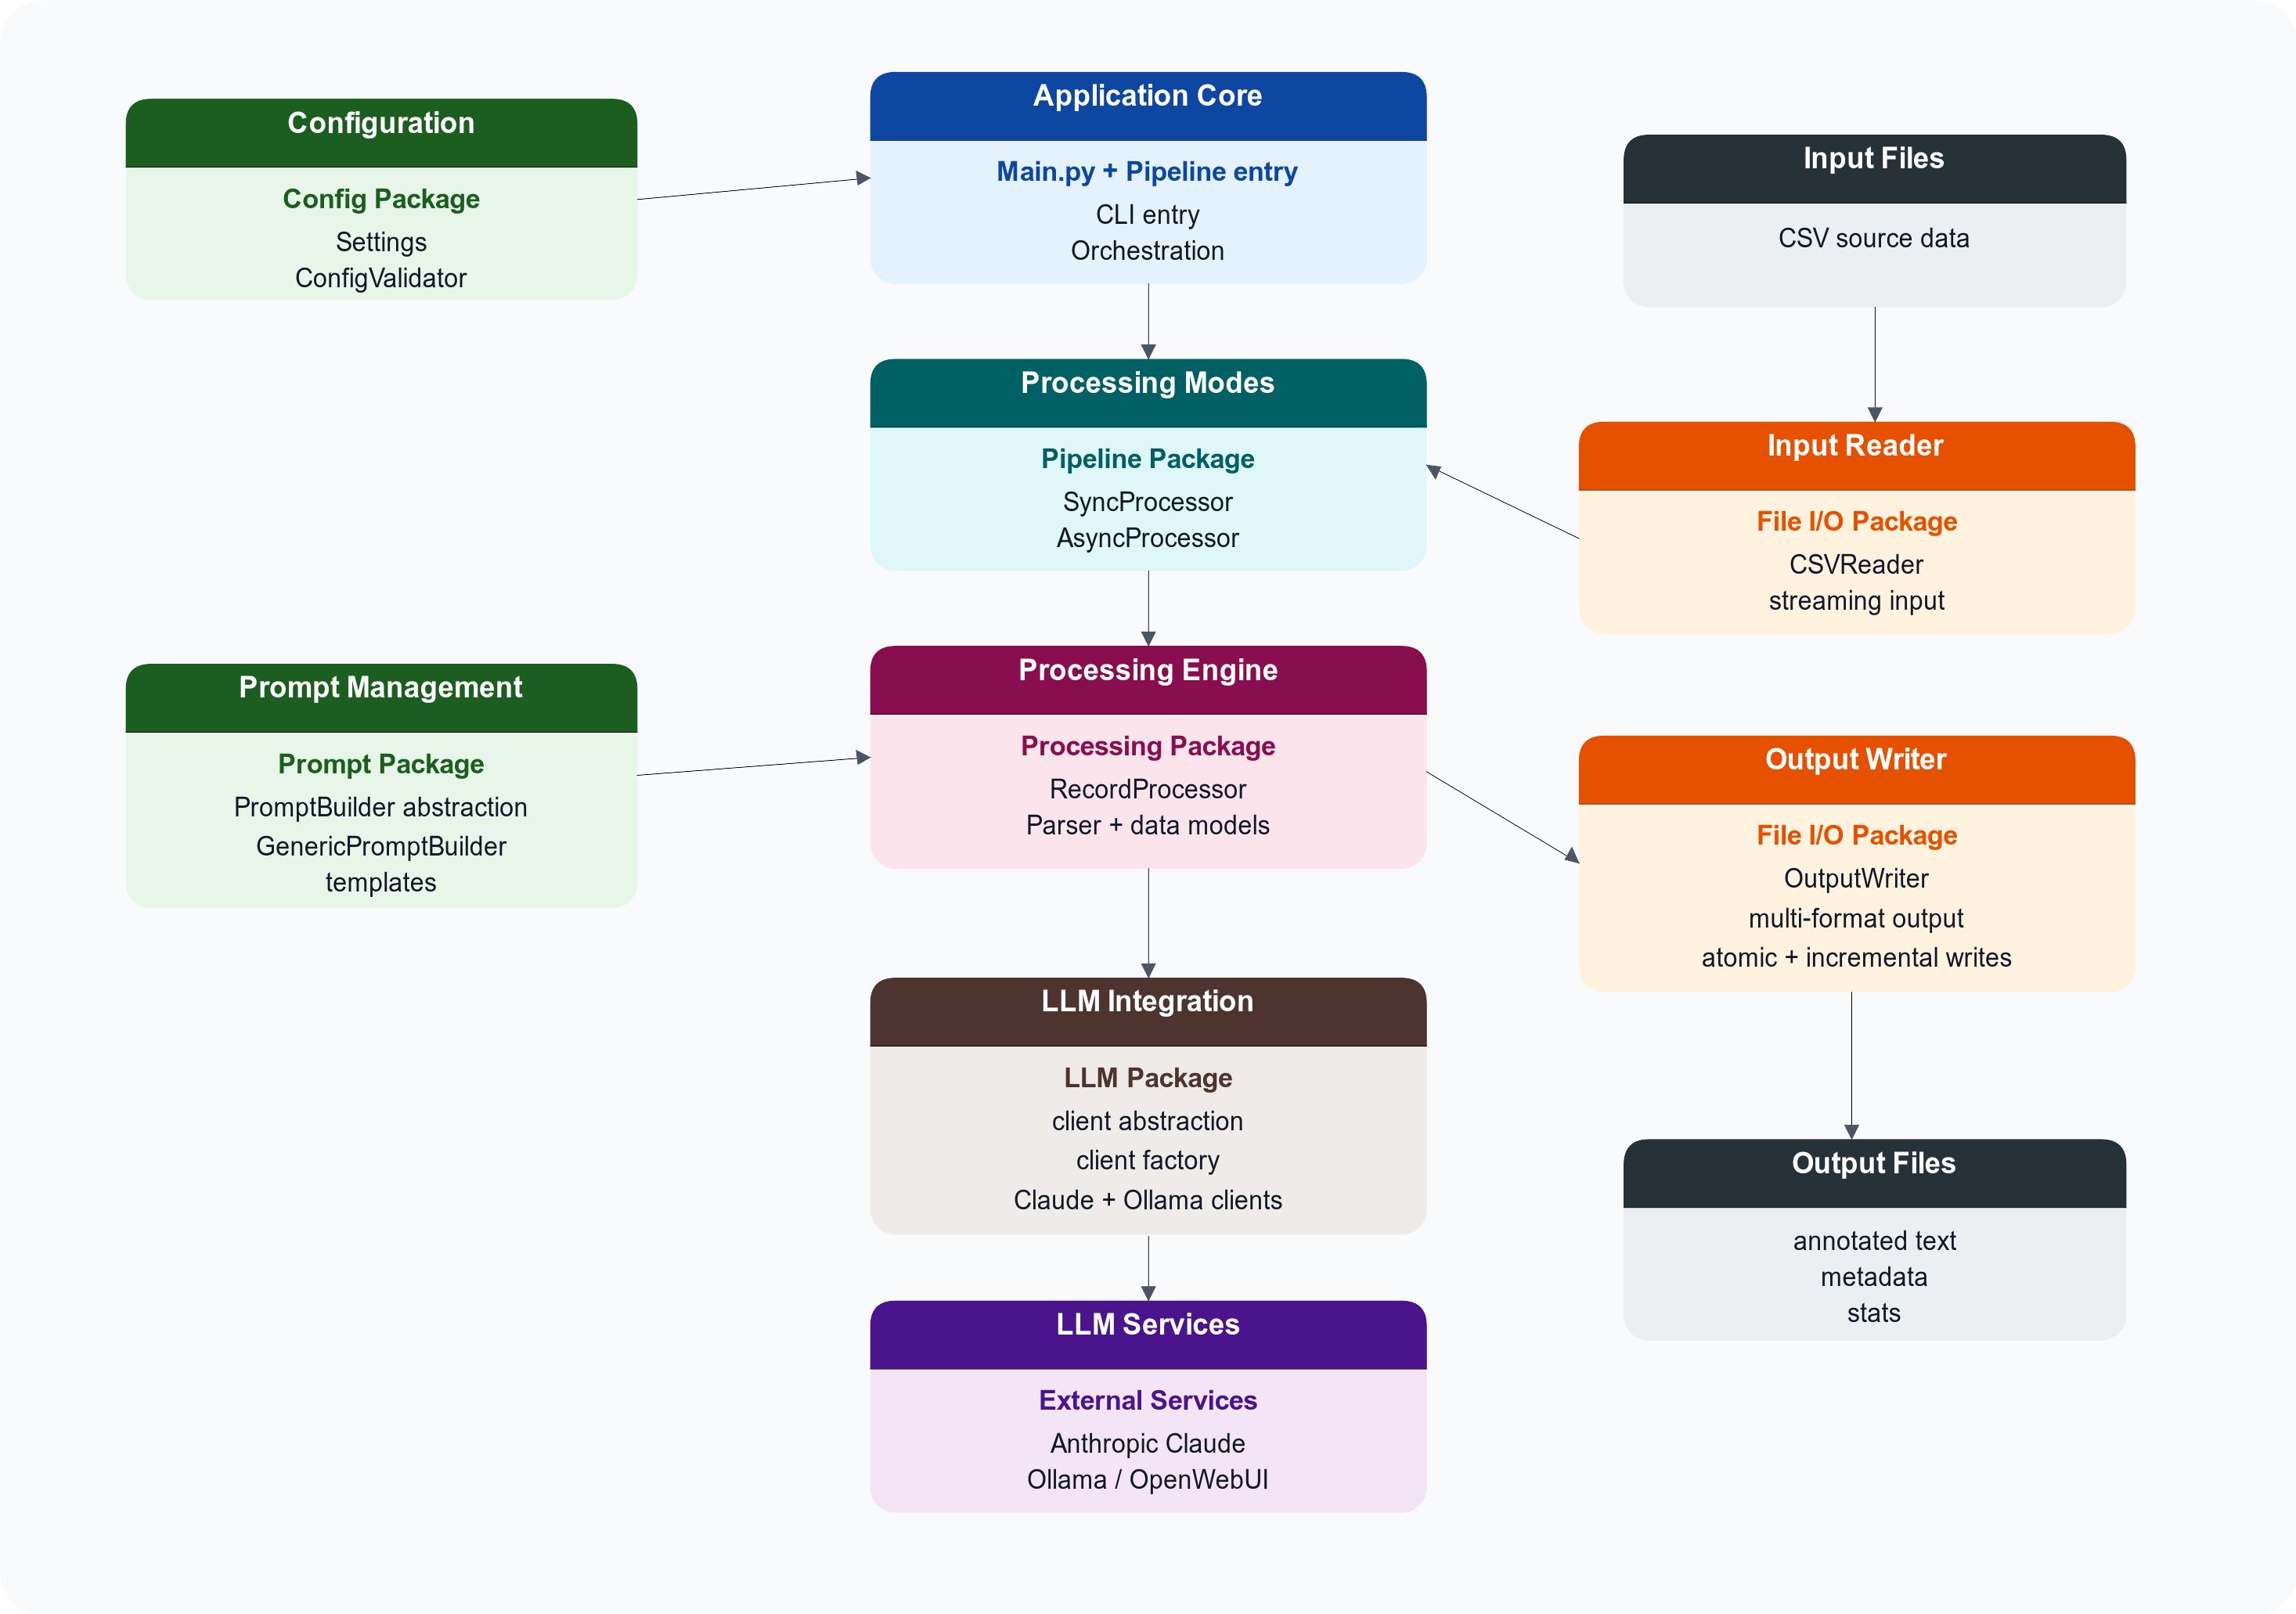
\includegraphics[width=1\textwidth,height=1\textheight,keepaspectratio]
    {../figs/ai-ner-system/architecture-overview-layered.png}
\end{frame}

\begin{frame}{Runtime Execution Flow}
  \slidefig{../figs/ai-ner-system/architecture-runtime-flow.png}
  \vspace{-0.4em}
  \scriptsize
  The application flows from CLI and configuration into pipeline orchestration,
  record processing, LLM calls, and final output files.
\end{frame}

\begin{frame}{Package-Oriented Architecture}
  \slidefig[0.8\textheight]{../figs/ai-ner-system/architecture-package-map.png}
  \vspace{-0.4em}
  \scriptsize
  \texttt{main.py} starts the app; the six packages divide configuration, I/O,
  prompts, LLM integration, processing logic, and orchestration responsibilities.
\end{frame}

\begin{frame}{End-to-End Record Journey}
  \slidefig{../figs/ai-ner-system/record-journey-flow.png}
  \vspace{-0.4em}
  \scriptsize
  One cleaned CSV row follows the same validate-build-call-parse path in both
  sync and async modes; the pipeline only changes orchestration and write
  strategy.
\end{frame}

\begin{frame}[shrink=4]{\texttt{main.py} Role and Startup Flow}
  \begin{columns}[T]
    \begin{column}{0.60\textwidth}
      \halfslidefig[0.9\textheight]{../figs/ai-ner-system/main-startup-flow.png}
    \end{column}
    \begin{column}{0.40\textwidth}
      \scriptsize
      \begin{itemize}
        \item \texttt{main.py} is the CLI entry point and top-level exit-code boundary.
        \vspace{1em}
        \item It builds the parser, parses arguments, configures logging, and performs quick argument checks.
        \vspace{1em}
        \item \texttt{\_validate\_configuration()} initializes \texttt{Settings}, applies CLI overrides, runs \texttt{ConfigValidator.validate\_all()}, and logs the effective configuration.
        \vspace{0.5em}
        \item \texttt{--dry-run} exits after full validation, before processor construction or any model call.
        \vspace{1em}
        \item On success, \texttt{main()} constructs \texttt{MedievalTextProcessor} and delegates execution.
      \end{itemize}
    \end{column}
  \end{columns}
\end{frame}

\begin{frame}[shrink=4]{Sync vs Async Dispatch and Processing Modes}
  \begin{columns}[T]
    \begin{column}{0.50\textwidth}
      \halfslidefig[0.9\textheight]{../figs/ai-ner-system/main-sync-async-dispatch.png}
    \end{column}
    \begin{column}{0.50\textwidth}
      \footnotesize
      \begin{itemize}
        \item \texttt{main.py} performs only the top-level sync vs async dispatch.
        \item Sync mode calls \texttt{processor.run()}, where the pipeline chooses individual processing or sync batch processing.
        \item Async mode creates a progress callback, then uses \texttt{asyncio.run(...)} to execute the \texttt{processor.run\_async(...)} coroutine.
        \item Inside async mode, the pipeline chooses concurrent individual processing or async batch orchestration, depending on client capability and options.
        \item So \texttt{main.py} owns CLI dispatch and event-loop entry; the pipeline owns the real execution strategy.
      \end{itemize}
    \end{column}
  \end{columns}
\end{frame}

\section{How the System Processes Text}

\begin{frame}[shrink=5]{Prompt Package Overview}
  \begin{columns}[T]
    \begin{column}{0.60\textwidth}
      \halfslidefig[0.90\textheight]{../figs/ai-ner-system/prompt-package-map.png}
    \end{column}
    \begin{column}{0.40\textwidth}
      \footnotesize
      \begin{itemize}
        \item The top-level \texttt{prompt/} folder stores the actual template files.
        \item The prompt package loads those files, extracts placeholders, and formats final prompts.
        \item The caller chooses the template file; \texttt{build(data)} dispatches by input shape inside \texttt{GenericPromptBuilder}.
        \item It normalizes source keys \texttt{Brevid}/\texttt{Tekst} to template keys \texttt{brevid}/\texttt{text} and checks required fields before formatting.
        \item \texttt{exceptions.py} defines prompt-specific template-load and prompt-build errors.
      \end{itemize}
    \end{column}
  \end{columns}
\end{frame}

\begin{frame}{Single-Record Template: \texttt{prompt.txt}}
  \begin{columns}[T]
    \begin{column}{0.60\textwidth}
      \begin{block}{Core Structure from \texttt{prompt.txt}}
        \footnotesize
        \begin{itemize}\setlength{\itemsep}{0.2em}
          \item \texttt{Brevid: \{brevid\}}
          \item \texttt{Text: """\{text\}"""}
          \item Task 1 marks up all proper nouns in the full medieval text as the format expression:\newline
          < name;type;preposition;order;brevid >.
          \item Task 2 returns \texttt{===JSON===} with entity metadata:
            \texttt{name}, \texttt{type}, \texttt{preposition}, \texttt{order},
            \texttt{description}, \texttt{brevid}, \texttt{gender}, and \texttt{language}.
        \end{itemize}
      \end{block}
    \end{column}
    \begin{column}{0.40\textwidth}
      \small
      \begin{itemize}
        \item The single-record template uses lowercase placeholders \texttt{\{brevid\}} and \texttt{\{text\}}.
        \item The output combines full annotated text and structured \texttt{===JSON===} metadata.
        \item It is used for sync single-record processing, async single-record processing, and async batch per-record requests.
      \end{itemize}
    \end{column}
  \end{columns}
\end{frame}

\begin{frame}{Sync Batch Template: \texttt{prompt-batch.txt}}
  \begin{columns}[T]
    \begin{column}{0.50\textwidth}
      \begin{block}{Core Structure from \texttt{prompt-batch.txt}}
        \footnotesize
        \begin{itemize}\setlength{\itemsep}{0.2em}
          \item Starts with strict output-format enforcement rules.
          \item Uses \texttt{\{num\_records\}} to declare the batch size.
          \item Uses \texttt{\{batch\_content\}} to inject all record payloads.
          \item Requires repeated \texttt{RECORD N RESULT} sections with
            annotated text plus \texttt{===JSON===} entity output.
        \end{itemize}
      \end{block}
    \end{column}
    \begin{column}{0.50\textwidth}
      \small
      \begin{itemize}
        \item The synchronous batch template uses \texttt{\{num\_records\}} and \texttt{\{batch\_content\}} placeholders.
        \item The builder assembles \texttt{batch\_content} as repeated \texttt{RECORD i}, \texttt{Brevid}, and \texttt{Text} input blocks.
        \item The response is structured as repeated \texttt{RECORD N RESULT} sections.
        \item It is only for synchronous multi-record prompting; Claude async batch still sends one prompt per record.
      \end{itemize}
    \end{column}
  \end{columns}
\end{frame}

\begin{frame}[shrink=12]{Prompt Flow in Code}
  \begin{columns}[T]
    \begin{column}{0.50\textwidth}
      \begin{block}{Template Path}
        \small
        \texttt{prompt/prompt.txt}\\
        \texttt{prompt/prompt-batch.txt}
      \end{block}
      \begin{block}{Builder Logic Pseudocode}
        \scriptsize
        \begin{algorithmic}
          \Procedure{Init}{template\_file}
            \State load template
          \EndProcedure
          \Statex
          \Procedure{Build}{data}
            \If{single record}
              \State extract template placeholders
              \State require \{brevid, text\} placeholders
              \State validate and clean record
              \State format and return final prompt
            \Else
              \State require non-empty record list
              \State extract template placeholders
              \State require \{num\_records, batch\_content\} placeholders
              \ForAll{records in batch}
                \State validate and clean record
              \EndFor
              \State assemble batch content
              \State format and return final prompt
            \EndIf
          \EndProcedure
        \end{algorithmic}
      \end{block}
    \end{column}
    \begin{column}{0.50\textwidth}
      \small
      \begin{itemize}
        \item The template file is chosen by the caller; \texttt{build(data)} dispatches by input shape.
        \item \texttt{build(data)} accepts either one record or a list of records.
        \item Single-record mode validates and formats \texttt{\{brevid\}} and \texttt{\{text\}}.
        \item Sync-batch mode validates \texttt{\{num\_records\}} and \texttt{\{batch\_content\}} and assembles repeated record blocks.
        \item Template loading fails early on missing, empty, non-file, or unreadable template files.
        \item Async batch still uses one single-record prompt per record.
      \end{itemize}
    \end{column}
  \end{columns}
\end{frame}

\begin{frame}[shrink=8]{Configuration Package}
  \begin{columns}[T]
    \begin{column}{0.5\textwidth}
      \halfslidefig[0.8\textheight]{../figs/ai-ner-system/config-settings-lifecycle.png}
    \end{column}
    \begin{column}{0.5\textwidth}
      \footnotesize
      \begin{itemize}
        \item \texttt{Settings} loads defaults and environment values into shared runtime configuration.
        \item \texttt{Settings.initialize()} can normalize paths, create output directories, and optionally validate common config.
        \item CLI overrides are applied afterward through \texttt{apply\_cli\_overrides()}, especially for input, output, and template paths.
        \item \texttt{ConfigValidator} is the pre-flight validation layer for client config, template/input files, and output path writability.
        \item \texttt{exceptions.py} defines the config error hierarchy for missing config, file problems, and directory problems.
      \end{itemize}
    \end{column}
  \end{columns}
\end{frame}

\begin{frame}{File I/O Package}
  \begin{columns}[T]
    \begin{column}{0.5\textwidth}
      \halfslidefig[0.8\textheight]{../figs/ai-ner-system/fileio-package-map.png}
    \end{column}
    \begin{column}{0.5\textwidth}
      \small
      \begin{itemize}
        \item \texttt{CSVReader} validates the input file, then streams cleaned semicolon-delimited rows.
        \item Required CSV headers can be validated when configured.
        \item \texttt{OutputWriter} writes three artifacts: annotated text, metadata table, and JSON stats.
        \item Text and metadata support atomic full writes and incremental writes with POSIX locked appends; stats use one final atomic JSON write.
        \item This package is the filesystem boundary of the application.
      \end{itemize}
    \end{column}
  \end{columns}
\end{frame}

\begin{frame}[shrink=5]{File I/O Runtime Logic}
  \begin{columns}[T]
    \begin{column}{0.5\textwidth}
      \begin{block}{CSVReader Logic Pseudocode}
        \scriptsize
        \begin{algorithmic}
          \Procedure{stream\_records}{}
            \State file already validated at construction
            \State open CSV file with configured delimiter and encoding
            \State create \texttt{csv.DictReader}
            \State capture headers
            \State validate required headers if configured
            \ForAll{rows in CSV}
              \If{row is empty}
                \State skip row
              \Else
                \State clean row values
                \State \textbf{yield} cleaned record
              \EndIf
            \EndFor
            \State wrap encoding, CSV, and OS errors as file I/O exceptions
          \EndProcedure
        \end{algorithmic}
      \end{block}
    \end{column}
    \begin{column}{0.5\textwidth}
      \begin{block}{\texttt{OutputWriter} Write Strategy}
        \scriptsize
        \begin{itemize}\setlength{\itemsep}{0.25em}
          \item Full text/metadata writes: build file content and atomically replace the target file.
          \item Incremental text/metadata writes: lock file, add header only if empty at lock time, add one separator newline if needed, append chunk, flush, unlock.
          \item Stats: serialize JSON and write one final atomic file.
          \item Locked append mode depends on POSIX \texttt{fcntl}, so it is not the cross-platform path.
        \end{itemize}
      \end{block}
      \begin{block}{Why This Design}
        \scriptsize
        \begin{itemize}\setlength{\itemsep}{0.25em}
          \item Streaming keeps input memory usage bounded.
          \item Atomic full writes avoid partially replaced output files.
          \item Locked appends let async processing emit ordered records safely during long runs.
        \end{itemize}
      \end{block}
    \end{column}
  \end{columns}
\end{frame}

\begin{frame}[shrink=12]{Pipeline Package}
  \begin{columns}[T]
    \begin{column}{0.6\textwidth}
      \halfslidefig[0.9\textheight]{../figs/ai-ner-system/pipeline-package-map.png}
    \end{column}
    \begin{column}{0.4\textwidth}
% MedievalTextProcessor:
% - initializes the shared runtime components: LLM client, prompt builder, RecordProcessor, CSVReader, and OutputWriter in main_processor.py (line 65)
% - owns output paths, headers, cleanup, and output finalization in main_processor.py (line 50) and main_processor.py (line 182)
% - exposes the two top-level execution entry points:
%    1. sync run() in main_processor.py (line 405)
%    2. async run_async() in main_processor.py (line 441)
% - delegates record processing to SyncProcessor / AsyncProcessor, but still owns timeout policy and final output writing in main_processor.py (line 419) and main_processor.py (line 479)
%
% delegates to:
%    - This means one component hands part of its work to another component.
%    - The meaning is: the pipeline-level processors do not perform the low-level NER business logic themselves. They delegate that record-level work to RecordProcessor
% typed against:
%    - This means the code depends on an interface/type contract, not directly on a concrete class.
%    ProcessorContext is effectively an interface-like abstraction, precisely in Python terms: it is a Protocol.
%    a Protocol is a typing-based interface so calling it an “interface” on a slide is reasonable.
%    it defines the small set of attributes and methods that SyncProcessor and AsyncProcessor need,
%    this lets them depend on that narrow contract instead of the whole concrete MedievalTextProcessor class.
%    MedievalTextProcessor is the concrete class that satisfies that protocol in practice, but the sub-processors only know about the protocol, not the concrete class.
%    - The meaning is: those classes are written to accept something that satisfies the ProcessorContext protocol, rather than depending on the concrete MedievalTextProcessor class directly.
      \scriptsize
      \begin{itemize}
        \item \texttt{MedievalTextProcessor} is the top-level runtime coordinator: it wires shared components, owns sync/async entry points, and handles output cleanup/finalization.
        \item \texttt{SyncProcessor} runs streaming synchronous execution, including individual mode, sync batch mode, and fallback handling.
        \item \texttt{AsyncProcessor} runs concurrent async execution with order preservation, incremental output, and batch progress monitoring.
        \item \texttt{processor\_protocol.py} defines \texttt{ProcessorContext}, a protocol-based interface so sub-processors depend on a narrow contract instead of the concrete main processor.
        \item \texttt{stats.py} holds async run statistics and the application-level error type.
      \end{itemize}
    \end{column}
  \end{columns}
\end{frame}

\begin{frame}{Processing Package}
  \begin{columns}[T]
    \begin{column}{0.6\textwidth}
      \halfslidefig[0.9\textheight]{../figs/ai-ner-system/processing-package-map.png}
    \end{column}
    \begin{column}{0.4\textwidth}
      \scriptsize
      \begin{itemize}
        \item This is the business-logic engine of the system.
        \item \texttt{RecordProcessor} orchestrates sync/async single-record and batch processing.
        \item \texttt{validator.py} checks input records, and \texttt{parser.py} converts raw LLM output into annotated text and entity metadata.
        \item \texttt{entities.py} defines \texttt{EntityRecord}, \texttt{ProcessingResult}, and \texttt{BatchProcessingResult}.
        \item \texttt{exceptions.py} centralizes the processing-layer error hierarchy.
      \end{itemize}
    \end{column}
  \end{columns}
\end{frame}

\begin{frame}{RecordProcessor Flow}
  \centering
  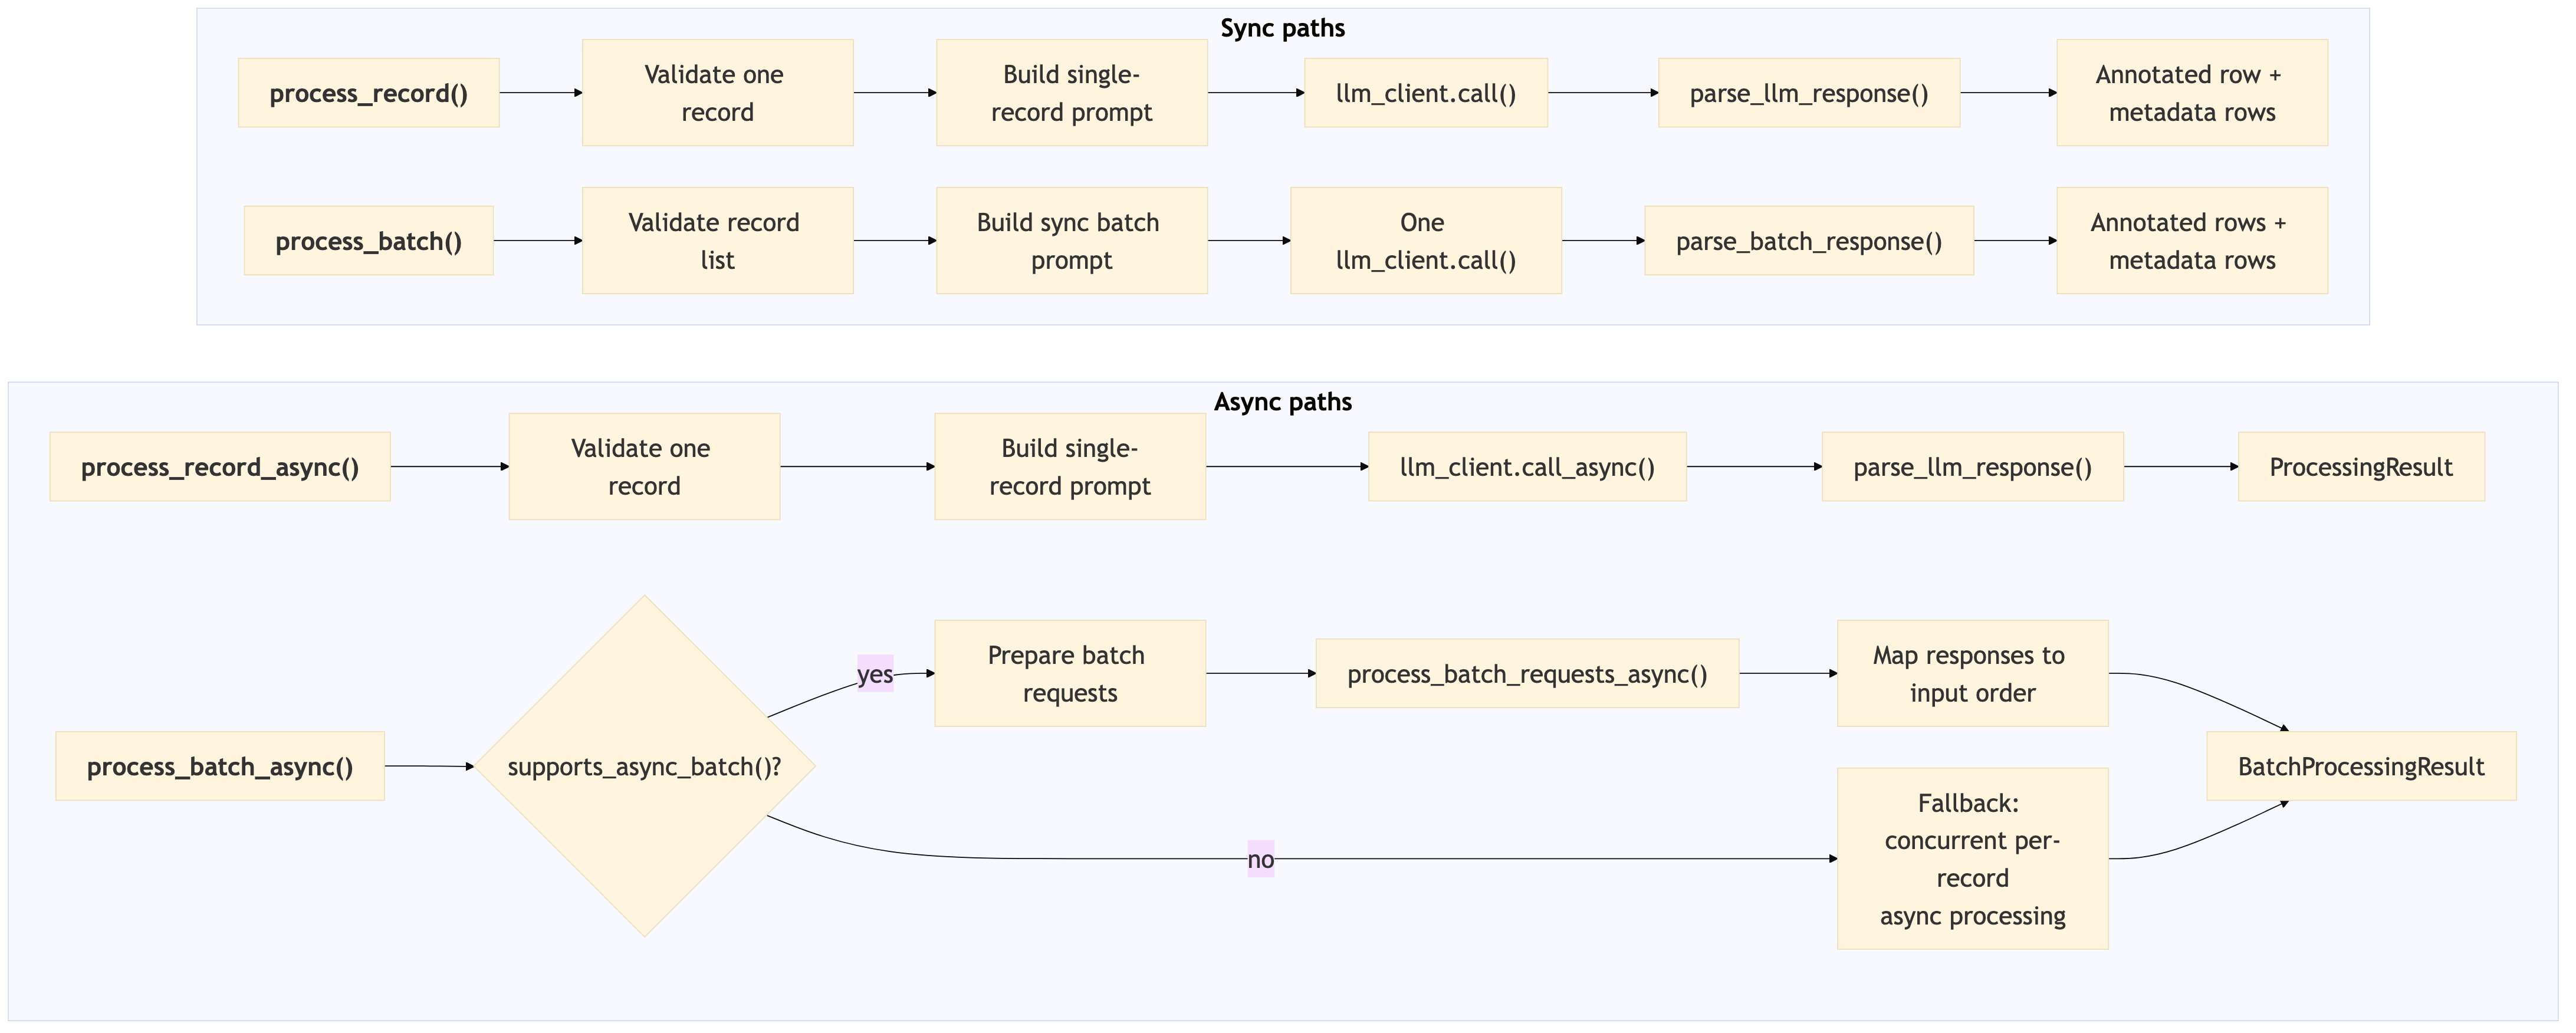
\includegraphics[width=\textwidth,height=0.80\textheight,keepaspectratio]
    {../figs/ai-ner-system/processing-recordprocessor-flow.png}
  \scriptsize
  Sync and async entry points share the same core stages: validate input, build prompts,
  call the LLM, parse responses, and package typed outputs.
\end{frame}

\begin{frame}{LLM Package}
  \begin{columns}[T]
    \begin{column}{0.5\textwidth}
      \halfslidefig[0.8\textheight]{../figs/ai-ner-system/llm-package-map.png}
    \end{column}
    \begin{column}{0.5\textwidth}
      \scriptsize
      \begin{itemize}
        \item The LLM package hides provider-specific APIs behind the shared \texttt{Client} abstraction.
        \item \texttt{base\_client.py} defines the common contract and shared async batch orchestration workflow.
        \item \texttt{ClaudeClient} is the full-featured adapter: sync, async, and async batch support.
        \item \texttt{OllamaClient} supports sync and async single requests, but not async batch.
        \item \texttt{batch\_models.py} and \texttt{exceptions.py} provide the shared batch contract and provider-level error hierarchy.
        \item \texttt{factory.py} creates the concrete client from validated settings.
      \end{itemize}
    \end{column}
  \end{columns}
\end{frame}

\section{From Sequential to Concurrent Execution}

\begin{frame}{Synchronous Pipeline Flow}
  \slidefig{../figs/ai-ner-system/pipeline-sync-flow.png}
  \vspace{-0.4em}
  \scriptsize
  \texttt{main\_processor.run()} cleans old outputs, then \texttt{SyncProcessor}
  streams records, falls back from failed batches to per-record processing, and
  writes output once at the end.
\end{frame}

\begin{frame}{Asynchronous Pipeline Flow}
  \slidefig{../figs/ai-ner-system/pipeline-async-flow.png}
  \vspace{-0.4em}
  \scriptsize
  \texttt{main\_processor.run\_async()} cleans old outputs, then
  \texttt{AsyncProcessor} chooses between concurrent per-record processing and
  provider-supported async batch streaming before final output is written.
\end{frame}

\begin{frame}{Async Batch Scheduler}
  \centering
  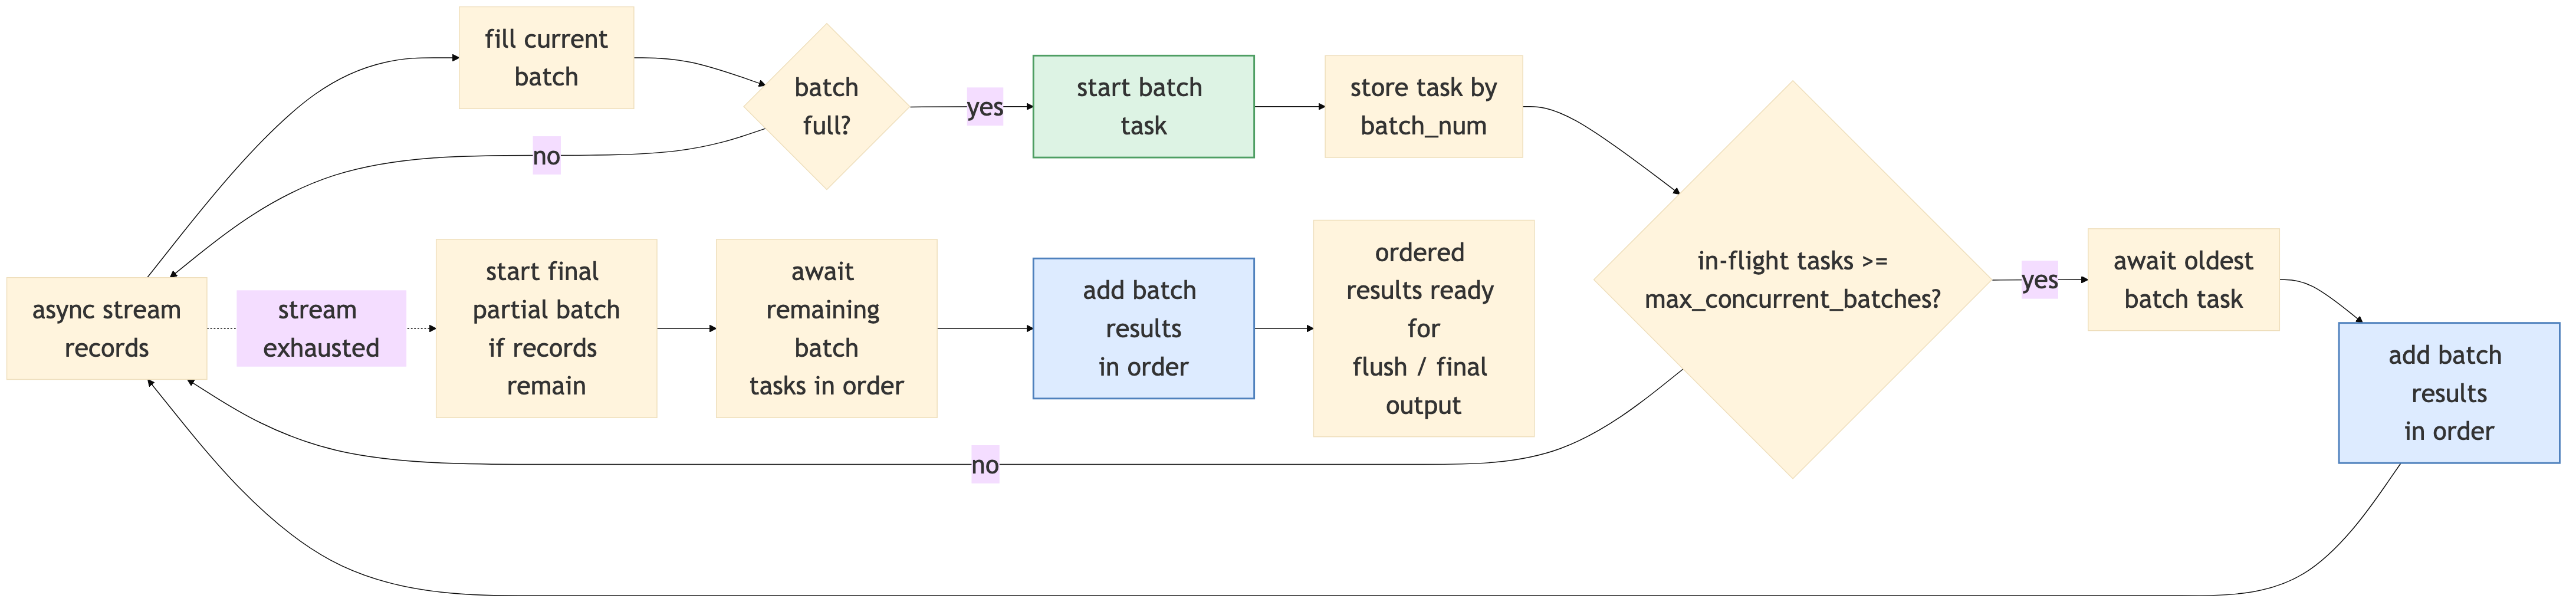
\includegraphics[width=\textwidth,height=0.78\textheight,keepaspectratio]
    {../figs/ai-ner-system/pipeline-async-batch-internals.png}
  \vspace{-0.3em}

  \scriptsize
  Step 1: fill batches, start tasks, and wait on the oldest task once the
  in-flight limit is reached. The next two slides zoom into the task body and
  ordered result handling.
\end{frame}

\begin{frame}{Async Batch Task Fallback}
  \centering
  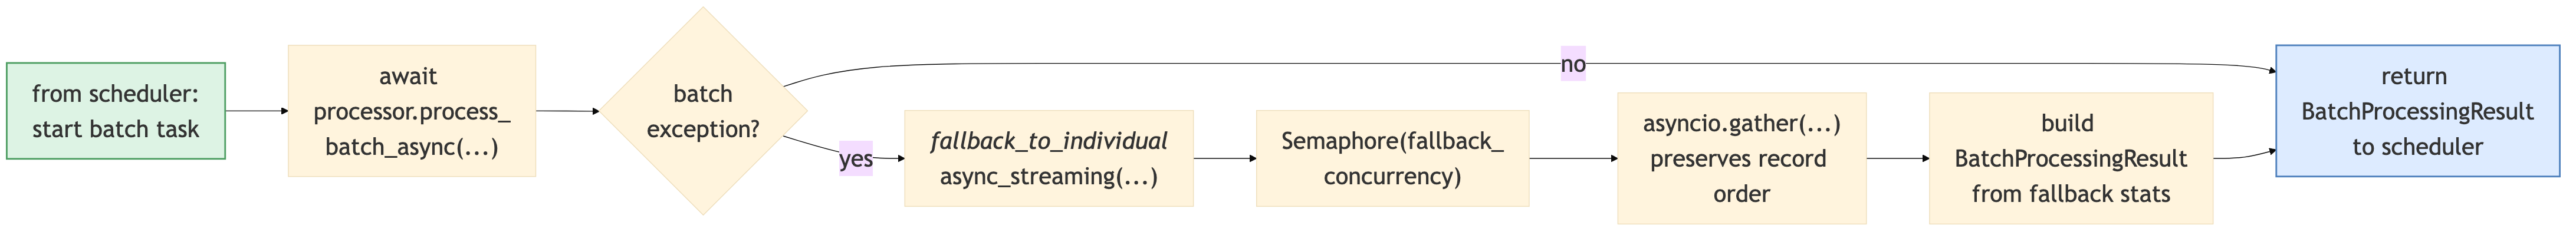
\includegraphics[width=\textwidth,height=0.72\textheight,keepaspectratio]
    {../figs/ai-ner-system/pipeline-async-batch-task-logic.png}
  \vspace{-0.2em}

  \scriptsize
  Step 2: each started task either returns a normal
  \texttt{BatchProcessingResult} or falls back to per-record async processing.
  Either way, the scheduler receives the same result shape: a completed batch
  result returned for ordered handling on the next slide.
\end{frame}

\begin{frame}{Async Batch Result Ordering}
  \centering
  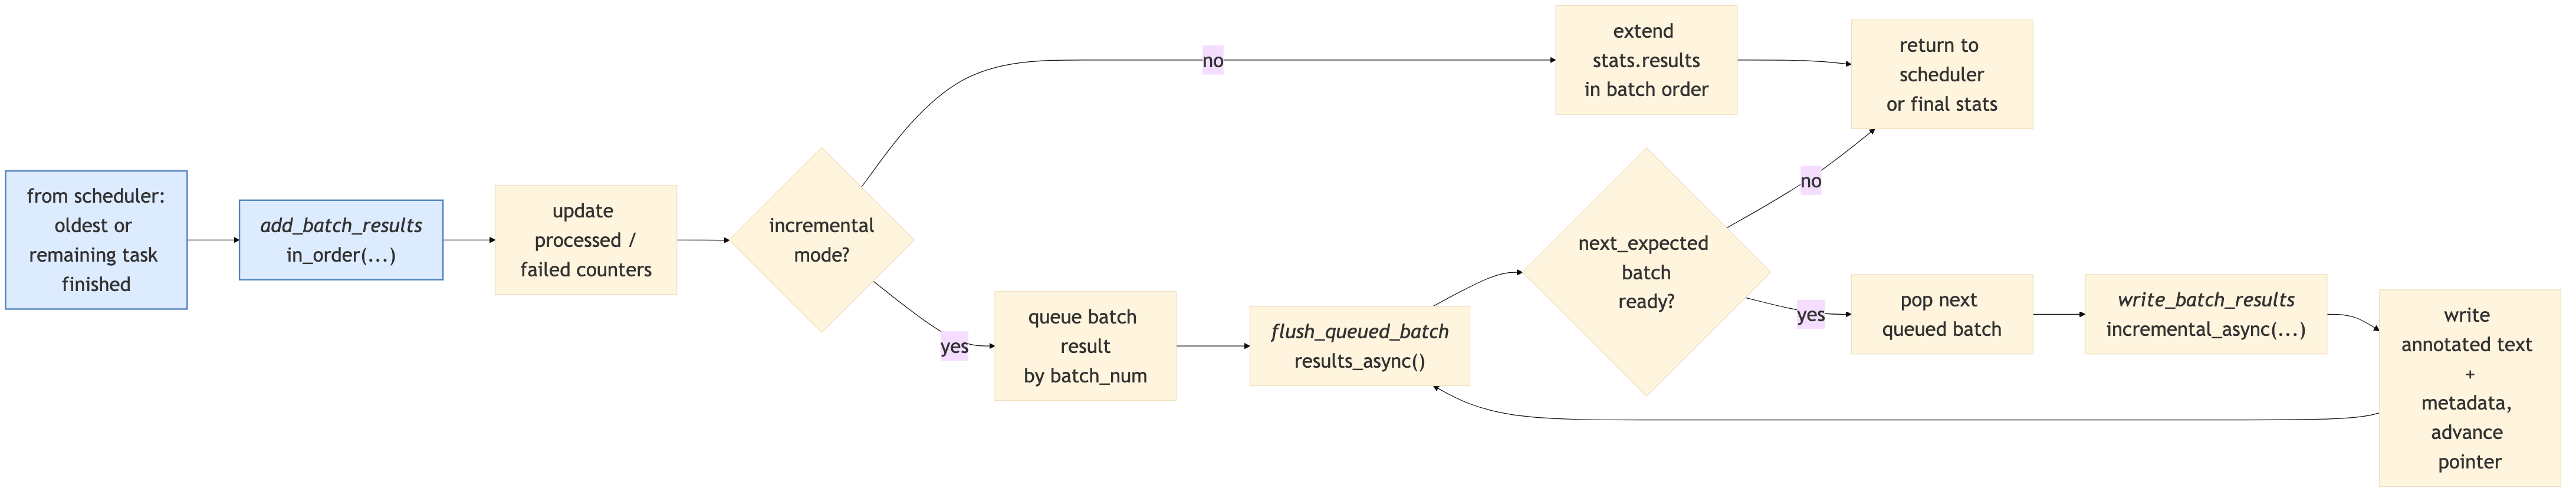
\includegraphics[width=\textwidth,height=0.68\textheight,keepaspectratio]
    {../figs/ai-ner-system/pipeline-async-batch-result-ordering.png}
  \vspace{-0.2em}

  \scriptsize
  \begin{itemize}\setlength{\itemsep}{0.2em}
    \item Step 3 starts when the scheduler receives a completed batch result and calls \texttt{\_add\_batch\_results\_in\_order()}.
    \item That method always updates counters before extending results or queueing the batch.
    \item In incremental mode, \texttt{\_flush\_queued\_batch\_results\_async()} may write multiple consecutive ready batches while \texttt{\_next\_expected\_batch\_num} advances.
  \end{itemize}
\end{frame}

\begin{frame}[shrink=2]{Async Batch Ordering Pseudocode}
  \begin{block}{Core Scheduling Logic}
    \scriptsize
    \begin{algorithmic}
      \Procedure{process\_records\_streaming\_async}{}
        \ForAll{streamed records}
          \State add record to current batch
          \If{batch full}
            \State start batch task and store by \texttt{batch\_num}
            \If{in-flight limit reached}
              \State await oldest batch task
              \State add results in order
            \EndIf
          \EndIf
        \EndFor
        \State start final partial batch if needed
        \ForAll{remaining batch tasks in order}
          \State await task
          \State add results in order
        \EndFor
        \If{incremental mode}
          \State flush queued next-expected batches
        \EndIf
      \EndProcedure
    \end{algorithmic}
  \end{block}
  \scriptsize
  \begin{itemize}\setlength{\itemsep}{0.1em}
    \item This condenses Step 1 and Step 3 into one control-flow view.
    \item Oldest-batch waiting preserves batch order while still allowing bounded concurrency.
    \item Failed batch tasks still return \texttt{BatchProcessingResult} after fallback, so the scheduler path stays uniform.
    \item Ordered flushing is separated from scheduling: ready batches are written only when their turn arrives.
  \end{itemize}
\end{frame}

\begin{frame}{Why Claude Async Batch Matters}
  \begin{columns}[T]
    \begin{column}{0.44\textwidth}
      \halfslidefig[0.64\textheight]{../figs/ai-ner-system/llm-async-batch-orchestration.png}
    \end{column}
    \begin{column}{0.52\textwidth}
      \footnotesize
      \begin{itemize}\setlength{\itemsep}{0.2em}
        \item The shared async-batch orchestration is \texttt{create -> wait \& poll -> fetch results} for one batch job.
        % \item Claude implements the async-batch primitives that this shared workflow depends on.
        \item Claude lets the pipeline submit multiple batches concurrently instead of waiting on one combined prompt at a time.
        \item Ollama does not implement that API shape, so higher layers must fall back to non-batch async strategies.
        \item This provider difference is one reason the LLM client abstraction matters.
      \end{itemize}
    \end{column}
  \end{columns}
\end{frame}

\section{Engineering and Results}

\begin{frame}[shrink=4]{Project Setup and Run Workflow}
  \begin{columns}[T]
    \begin{column}{0.45\textwidth}
      \footnotesize
      \begin{itemize}\setlength{\itemsep}{0.3em}
        \item Install dependencies with \texttt{uv sync}.
        \item Copy \texttt{.env.example} to \texttt{.env} and add Claude API or OpenWebUI/Ollama credentials.
        \item Default client, paths, and templates come from settings and environment values; CLI flags can override them for custom runs.
        \item \texttt{--dry-run} performs full argument, config, file, and client validation without processing.
        \item Async mode also exposes tuning flags for concurrency, chunking, polling, wait limits, and incremental output.
      \end{itemize}
    \end{column}
    \begin{column}{0.55\textwidth}
      \begin{block}{Common Run Profiles}
        \scriptsize
        \begin{itemize}\setlength{\itemsep}{0.2em}
          \item \textbf{Sync individual}: default path
          \item \textbf{Sync batch}: \texttt{--use-batch} + \texttt{--batch-size N}
          \item \textbf{Async individual}: \texttt{--async-mode}
          \item \textbf{Async batch}: \texttt{--async-mode} + \texttt{--batch-size N}
        \end{itemize}
      \end{block}
      \scriptsize
      % \ttfamily\tiny
      Async batch still depends on provider capability: Claude supports it; Ollama falls back to non-batch async execution.
      \begin{block}{Example Commands}
        \ttfamily\tiny
        \textrm{\# Validate without processing}\\
        uv run -m ai\_ner\_system.main\\
        \hspace*{1em}--client claude --dry-run\\[0.3em]
        \textrm{\# Sync batch processing}\\
        uv run -m ai\_ner\_system.main\\
        \hspace*{1em}--client ollama --use-batch\\
        \hspace*{1em}--batch-size 10\\[0.3em]
        \textrm{\# Async batch (production)}\\
        uv run -m ai\_ner\_system.main\\
        \hspace*{1em}--client claude --async-mode\\
        \hspace*{1em}--batch-size 100\\
        \hspace*{1em}--incremental-output
      \end{block}
    \end{column}
  \end{columns}
\end{frame}

\begin{frame}{Project Tooling}
  \begin{columns}[T]
    \begin{column}{0.52\textwidth}
      \begin{block}{Runtime and Packaging}
        \scriptsize
        \begin{itemize}\setlength{\itemsep}{0.3em}
          \item Python requirement is \texttt{>=3.11}; CI also runs on 3.12 and 3.13.
          \item \texttt{uv} is the primary workflow for environment setup, dependency sync, and command execution.
          \item \texttt{pyproject.toml} is the single source of truth for package metadata, dependencies, entry points, and developer tooling.
          \item \texttt{uv.lock} pins resolved versions for reproducible environments and safer dependency updates.
          \item The CLI can run as \texttt{uv run ai-ner-system ...} instead of the module form.
        \end{itemize}
      \end{block}
    \end{column}
    \begin{column}{0.48\textwidth}
      \begin{block}{Dependency and Workflow Groups}
        \scriptsize
        \begin{itemize}\setlength{\itemsep}{0.3em}
          \item Core runtime dependencies include \texttt{python-dotenv}, \texttt{anthropic}, \texttt{aiohttp}, and \texttt{requests}; \texttt{asyncio} comes from the Python standard library.
          \item Project extras expose install profiles such as \texttt{lint}, \texttt{test}, \texttt{security}, and combined \texttt{ci}.
          \item \texttt{uv} also defines development groups for the main engineering workflows used for this project.
          \item Static analysis and pytest behavior are configured centrally in \texttt{pyproject.toml}; the next slide shows how those checks run in practice.
        \end{itemize}
      \end{block}
    \end{column}
  \end{columns}
\end{frame}

\begin{frame}{Testing and Quality Assurance}
  \begin{columns}[T]
    \begin{column}{0.50\textwidth}
      \begin{block}{Quality Toolchain}
        \scriptsize
        \begin{itemize}\setlength{\itemsep}{0.3em}
          \item \textbf{Ruff} — lint + format checks
          \item \textbf{MyPy + Pyright} — static typing
          \item \textbf{Pytest + pytest-asyncio} — unit and async tests
          \item \textbf{Pre-commit} — local gate before CI
        \end{itemize}
      \end{block}
      \vspace{0.3em}
      \begin{block}{CI and Repo Safeguards}
        \scriptsize
        \begin{itemize}\setlength{\itemsep}{0.2em}
          \item Push/PR CI runs Ruff, MyPy, and unit tests with coverage on Python 3.11 / 3.12 / 3.13, then uploads coverage to Codecov.
          \item Separate workflows run Bandit, Safety, and CodeQL.
          \item GitHub safeguards include Dependabot alerts, code scanning alerts, and code quality findings.
        \end{itemize}
      \end{block}
    \end{column}
    \begin{column}{0.50\textwidth}
      \begin{block}{Coverage Snapshot by Package}
        \scriptsize
        \begin{tabular}{lr}
          \texttt{config}      & 95--100\% \\
          \texttt{file\_io}    & 94--100\% \\
          \texttt{llm}         & 95--100\% \\
          \texttt{processing}  & 100\% \\
          \texttt{prompt}      & 90--99\% \\
          \midrule
          \texttt{pipeline}    & 0\% \\
          \texttt{main.py}     & 0\% \\
        \end{tabular}
      \end{block}
      \vspace{0.3em}
      \scriptsize
      \begin{itemize}\setlength{\itemsep}{0.3em}
        \item Latest recorded unit-test coverage is about 69\% overall; five core packages are at 90--100\%.
        \item \texttt{pipeline} and \texttt{main.py} are still the weakest areas because orchestration logic needs more direct tests.
      \end{itemize}
    \end{column}
  \end{columns}
\end{frame}

\begin{frame}[shrink=4]{Performance Benchmarks}
  \begin{columns}[T]
    \begin{column}{0.55\textwidth}
      \begin{block}{Benchmark Results (\textasciitilde18\,559 record corpus)}
        \scriptsize
        \resizebox{\linewidth}{!}{%
          \begin{tabular}{lcccccc}
            \toprule
            Mode & Provider & Records & Time & Throughput & Cost & Projected \\
            \midrule
            Sync individual & \textbf{Ollama/Gemma3} & 10  & 6:15  & 1.6 rec/min & \$0.31 & \textasciitilde194\,h \\
            Sync batch (size 10) & \textbf{Ollama/Gemma3} & 10  & 5:23  & 1.9 rec/min & \$0.29 & \textasciitilde161\,h \\
            Async batch (size 10)  & \textbf{Claude/sonnet4} & 10  & 1:34  & 6.4 rec/min & \$0.17 & \textasciitilde47\,h \\
            Async batch (size 100) & \textbf{Claude/sonnet4}  & 551 & 13:47 & 40 rec/min & \textasciitilde\$12 & \textasciitilde7.7\,h \\
            \bottomrule
          \end{tabular}%
        }
      \end{block}
      \vspace{0.3em}
      \scriptsize
      \begin{itemize}\setlength{\itemsep}{0.2em}
        \item These benchmarks compare both execution mode and provider/model, not batching strategy alone.
        \item The 551-record async row is a scale trial; the other rows are small-sample runs.
        \item Claude async batch shows the largest measured throughput gain, time reduction, and lower cost per record at scale.
        \item Architecture choice here affects runtime, cost, and feasible corpus-scale execution.
      \end{itemize}
    \end{column}
    \begin{column}{0.45\textwidth}
      \begin{block}{Projected Full-Corpus Time}
        \centering
        \scriptsize
        \vspace{0.3em}
        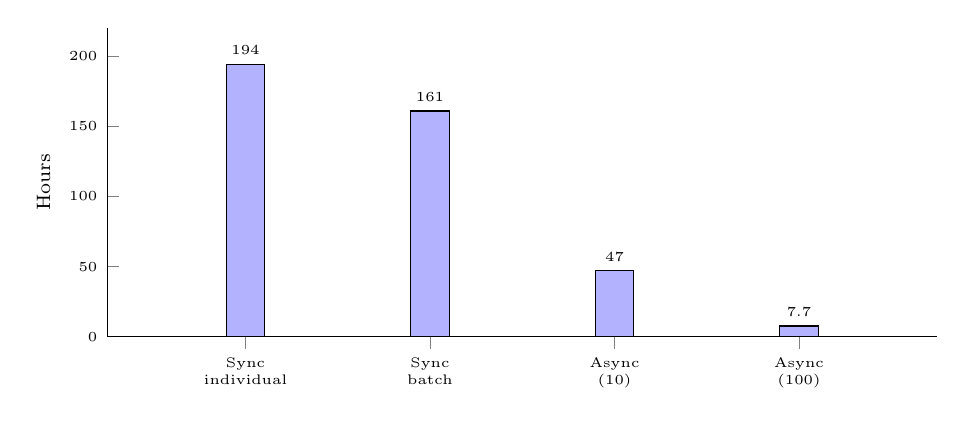
\begin{tikzpicture}
          \begin{axis}[
            ybar,
            bar width=14pt,
            width=\linewidth,
            height=5.5cm,
            ylabel={Hours},
            ylabel style={font=\scriptsize},
            xtick={1,2,3,4},
            xticklabels={{Sync\\individual},{Sync\\batch},{Async\\(10)},{Async\\(100)}},
            xticklabel style={font=\tiny, align=center},
            yticklabel style={font=\tiny},
            ymin=0, ymax=220,
            nodes near coords,
            every node near coord/.style={font=\tiny, above},
            axis lines*=left,
            enlarge x limits=0.25,
          ]
            \addplot[
              fill=blue!30,
              point meta=explicit symbolic,
            ] coordinates {
              (1,194)  [194]
              (2,161)  [161]
              (3,47)   [47]
              (4,7.7)  [7.7]
            };
          \end{axis}
        \end{tikzpicture}
        \vspace{-0.3em}
      \end{block}
    \end{column}
  \end{columns}
\end{frame}

\begin{frame}{Anthropic API Rate Limits}
  \begin{columns}[T]
    \begin{column}{0.55\textwidth}
      \begin{block}{Claude API Limits (Tier 2)}
        \scriptsize
        \begin{tabular}{lr}
          \multicolumn{2}{l}{\textbf{Message Batches API}} \\
          \midrule
          Requests per batch (max)              & 100K \\
          Requests in processing queue          & 200K \\
          Management endpoint calls/min         & 1K \\[0.5em]
          \multicolumn{2}{l}{\textbf{Messages API (per model)}} \\
          \midrule
          Requests per minute                   & 1K \\
          Input tokens per minute               & 450K \\
          Output tokens per minute              & 90K \\[0.5em]
          \multicolumn{2}{l}{\textbf{Spend}} \\
          \midrule
          Monthly spend limit                   & \$500 \\
        \end{tabular}
      \end{block}
    \end{column}
    \begin{column}{0.45\textwidth}
      \begin{block}{Batch vs Management Calls}
        \scriptsize
        A batch contains up to 100K requests, but creating, polling, and
        retrieving that batch are \textbf{management calls} (1K/min limit).
        The batch contents are processed asynchronously by Anthropic's servers.
      \end{block}
      \vspace{0.2em}
      \scriptsize
      These Tier 2 limits are taken from the current Anthropic docs/console and may vary by organization or tier.
    \end{column}
  \end{columns}
\end{frame}

\begin{frame}{Concurrency Design for Staying Within API Limits}
  \begin{columns}[T]
    \begin{column}{0.50\textwidth}
      \begin{block}{Batch Async Path (Batches API)}
        \scriptsize
        \begin{itemize}\setlength{\itemsep}{0.3em}
          \item \textbf{Bounded batch concurrency}:
            \texttt{max\_concurrent\_batches} (default 5) caps in-flight batch jobs.
            The scheduler awaits the oldest batch before starting a new one.
          \item \textbf{Poll-based progress monitoring}:
            \texttt{poll\_interval} (default 30\,s) controls how often each batch checks its status via the management API.
          \item \textbf{Fallback concurrency}:
            \texttt{fallback\_concurrency} (default 3) limits parallelism when a failed batch retries records individually.
        \end{itemize}
      \end{block}
    \end{column}
    \begin{column}{0.50\textwidth}
      \begin{block}{Individual Async Path (Messages API)}
        \scriptsize
        \begin{itemize}\setlength{\itemsep}{0.3em}
          \item \textbf{Semaphore-limited concurrency}:
            \texttt{max\_concurrent\_individual} (default 5) bounds concurrent per-record API calls.
          \item \textbf{Chunk-based memory management}:
            \texttt{chunk\_size} (default 50) limits how many tasks accumulate before awaiting results together.
        \end{itemize}
      \end{block}
      \vspace{0.2em}
      \begin{block}{Management API Call Budget}
        \ttfamily\tiny
        Each poll = 2 API calls (\texttt{status check} + \texttt{batch info}).
        At \texttt{poll\_interval=30s}, each batch polls 2 polls/min. With 5 concurrent batches:\\[0.3em]
        \centering
        5\,batches $\times$ 2\,calls/poll $\times$ 2\,polls/min = 20\,calls/min\\
        (2\% of 1K management limit)
      \end{block}
    \end{column}
  \end{columns}
  \centering
  \scriptsize
  All defaults are in \texttt{Settings} and overridable via CLI flags.
\end{frame}

\begin{frame}[shrink=6]{Candidate Optimized Settings for Full-Corpus Execution}
  \scriptsize
  These are modeled candidate settings from the current benchmarks and API limits, not yet validated by a full-corpus run.
  \begin{columns}[T]
    \begin{column}{0.50\textwidth}
      \begin{block}{Default vs Optimized Settings}
        \scriptsize
        \begin{tabular}{lrr}
          & \textbf{Default} & \textbf{Optimized} \\
          \midrule
          \texttt{batch\_size}      & 5       & \textbf{200} \\
          \texttt{max\_conc.\_b.}  & 5       & \textbf{8}   \\
          \texttt{poll\_interval}   & 30\,s   & \textbf{20\,s} \\
          \texttt{chunk\_size}      & 50      & \textbf{100} \\
          \texttt{fallback\_conc.}  & 3       & 3 \\
        \end{tabular}
      \end{block}
      \vspace{0.2em}
      \begin{block}{Why These Values Are Safe}
        \scriptsize
        \begin{itemize}\setlength{\itemsep}{0.2em}
          \item \texttt{batch\_size=200}: 0.2\% of the 100K/batch limit.
            Creates about 93 batches for 18,559 records.
          \item \texttt{max\_concurrent\_batches}=8: at most 1,600 records in
            queue (0.8\% of 200K limit).
          \item Management API usage: $\sim$56 calls/min
            (5.6\% of 1K limit).
          \item Estimated cost: $\sim$\$396
            (within the \$500/month Tier~2 cap).
        \end{itemize}
      \end{block}
    \end{column}
    \begin{column}{0.50\textwidth}
      \begin{block}{Projected Full-Corpus Time}
        \centering
        \scriptsize
        \vspace{0.3em}
        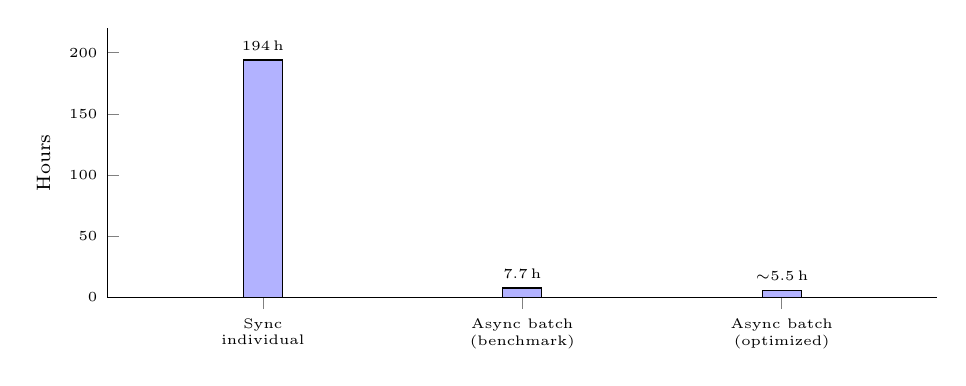
\begin{tikzpicture}
          \begin{axis}[
            ybar,
            bar width=14pt,
            width=\linewidth,
            height=5.0cm,
            ylabel={Hours},
            ylabel style={font=\scriptsize},
            xtick={1,2,3},
            xticklabels={
              {Sync\\individual},
              {Async batch\\(benchmark)},
              {Async batch\\(optimized)}},
            xticklabel style={font=\tiny, align=center},
            yticklabel style={font=\tiny},
            ymin=0, ymax=220,
            nodes near coords,
            every node near coord/.style={font=\tiny, above},
            axis lines*=left,
            enlarge x limits=0.3,
          ]
            \addplot[
              fill=blue!30,
              point meta=explicit symbolic,
            ] coordinates {
              (1,194)   [194\,h]
              (2,7.7)   [7.7\,h]
              (3,5.5)   [{$\sim$5.5\,h}]
            };
          \end{axis}
        \end{tikzpicture}
        \vspace{-0.3em}
      \end{block}
      \vspace{0.2em}
      \scriptsize
      \begin{itemize}\setlength{\itemsep}{0.2em}
        \item Benchmark (batch 100, 5 concurrent): 40\,rec/min.
        \item Optimized (batch 200, 8 concurrent, 20\,s poll):
          projected $\sim$55\,rec/min $\rightarrow$ \textbf{$\sim$5--6\,hours}.
      \end{itemize}
    \end{column}
  \end{columns}
\end{frame}

\begin{frame}{Annotated Output Example}
  \scriptsize
  Sample annotated text from a Claude async incremental run
  (\texttt{13} records, \texttt{batch\_size=2}).
  \vspace{0.3em}
  \begin{block}{Annotated Text Excerpt (Brevid 601)}
    \ttfamily\scriptsize
    ... sændir \textless{} Olauer;Person Name;N/A;1;601 \textgreater{}\\
    med gudz nadh abote j \textless{} Olafsklaustre;Place Name;j;2;601 \textgreater{}\\
    j \textless{} Tunsbergi;Place Name;j;3;601 \textgreater{} q. g. ok sina kunnikt gerande ...\\[0.3em]
    ... opno brefue a \textless{} Olafsklausters;Place Name;a;4;601 \textgreater{} vægna þet ...\\
    ... sæm sira \textless{} Æirikar Kolbiornason;Person Name;N/A;5;601 \textgreater{}\\
    prester a \textless{} Sondum;Place Name;a;6;601 \textgreater{} hafde kœypt ...
  \end{block}
  \scriptsize
  Inline tags preserve the original text and add
  \texttt{\textless{} name; type; preposition; order; brevid \textgreater{}}.
\end{frame}

\begin{frame}[shrink=2]{Metadata Output Example}
  \scriptsize
  Sample metadata rows from the same Claude async incremental run.
  \vspace{0.3em}
  \begin{block}{Selected Metadata Rows}
    \ttfamily\scriptsize
    Entity;Type;Preposition;Order;Brevid;Description;Gender;Language\\
    Olauer;Person Name;N/A;1;601;Abbot;Male;non\\
    Olafsklaustre;Place Name;j;2;601;Monastery;N/A;non\\
    Tunsbergi;Place Name;j;3;601;Town/City;N/A;non\\
    Olafsklausters;Place Name;a;4;601;Monastery;N/A;non\\
    Æirikar Kolbiornason;Person Name;N/A;5;601;Priest;Male;non\\
    Sondum;Place Name;a;6;601;Location;N/A;non
  \end{block}
  \scriptsize
  One semicolon-delimited row is written for each extracted entity.
\end{frame}

\begin{frame}{Future Work}
  \begin{columns}[T]
    \begin{column}{0.50\textwidth}
      \begin{block}{Short-term}
        \scriptsize
        \begin{enumerate}\setlength{\itemsep}{0.3em}
          \item Add direct tests for pipeline orchestration and \texttt{main.py} paths.
          \item Validate candidate optimized async-batch settings on the full 18,559-record corpus.
          \item Evaluate output quality through domain review and structured error analysis.
          \item Measure production-scale cost, throughput, and fallback behavior.
        \end{enumerate}
      \end{block}
    \end{column}
    \begin{column}{0.50\textwidth}
      \begin{block}{Long-term}
        \scriptsize
        \begin{enumerate}\setlength{\itemsep}{0.3em}
          \item Add smarter retry/backoff and adaptive rate-limit handling for provider APIs.
          \item Expand integration/system testing for full sync/async workflows.
          \item Explore \textbf{harness engineering}\footnotemark{} to build
            an agentic architecture for medieval-text processing with reusable
            orchestration and experiment workflows.
          \item Integrate the pipeline with a frontend or dashboard for
            easier monitoring and result inspection.
        \end{enumerate}
      \end{block}
    \end{column}
  \end{columns}
  \footnotetext{
    \tiny
    Harness engineering: reusable orchestration, tool integration, and context management for agentic systems.
  }
\end{frame}
\end{document}
